\documentclass[a4paper]{article}

\usepackage[T2A]{fontenc}
\usepackage[utf8]{inputenc}
\usepackage[russian]{babel}


\usepackage{graphicx}
\usepackage{float}
\usepackage{mathtools}
\usepackage{wrapfig}
\usepackage{amsfonts, amssymb, amsmath, latexsym}
\usepackage{nicefrac}
\usepackage{hhline}
\usepackage{multirow}
\usepackage[colorinlistoftodos,bordercolor=orange,backgroundcolor=orange!20,linecolor=orange,textsize=scriptsize]{todonotes}
\usepackage[colorlinks=true,linkcolor=blue,citecolor=blue]{hyperref}       % hyperlinks
\usepackage{nicefrac}       % compact symbols for 1/2, etc.
\usepackage{nameref}
\usepackage{booktabs}       % professional-quality tables

\usepackage{algorithm}
\usepackage{algpseudocode}

\usepackage{xcolor, colortbl}
\usepackage{etoolbox}

% \graphicspath{ {./} }

\usepackage[verbose=true,letterpaper]{geometry}

\newgeometry{
    textheight=9in,
    textwidth=5.5in,
    top=1in,
    headheight=12pt,
    headsep=25pt,
    footskip=30pt
}

\usepackage{epigraph}

%

\usepackage{amsmath,amsfonts,amssymb,amsthm,mathtools, mathrsfs}
\newcommand{\argmin}{\mathop{\arg\!\min}}
\newcommand{\argmax}{\mathop{\arg\!\max}}

\newcommand{\Var}{\mathbb{V}}
\newcommand{\Exp}{\mathbb{E}}
\newcommand{\Cov}{\text{Cov}}
\newcommand{\makebold}[1]{\boldsymbol{#1}}
\newcommand{\mean}[1]{\overline{#1}}
\newcommand{\eps}{\varepsilon}
\renewcommand{\epsilon}{\varepsilon}

\newcommand{\partfrac}[2]{\frac{\partial #1}{\partial #2}}
\newcommand{\ttt}[1]{\texttt{#1}}
\newcommand{\term}[1]{\textbf{#1}}

\newcommand{\la}{\langle}
\newcommand{\ra}{\rangle}

\newcommand{\lp}{\left(}
\newcommand{\rp}{\right)}
\newcommand{\lf}{\left\{}
\newcommand{\rf}{\right\}}
\newcommand{\ls}{\left[}
\newcommand{\rs}{\right]}
\newcommand{\lv}{\left|}
\newcommand{\rv}{\right|}

\newcommand*{\affaddr}[1]{#1} % No op here. Customize it for different styles.
\newcommand*{\affmark}[1][*]{\textsuperscript{#1}}


\usepackage{amsthm}

\theoremstyle{definition}
\newtheorem{definition}{Определение}[section]

\newtheorem{exercise}{Задача}[section]

\newtheorem*{solution}{Решение}
\theoremstyle{remark}
\newtheorem*{remark}{Remark}

\makeatletter
\renewcommand{\l@section}{\@dottedtocline{1}{0em}{2.1em}}
\makeatother

% \setlength\epigraphwidth{.8\textwidth}
\setlength\epigraphrule{0pt}

\title{Работа 3.3.4 \\ Эффект Холла в полупроводниках}
\author{Шарапов Денис, Зелёный Николай, Б05-005}
\date{}

\usepackage{fancyhdr}
\pagestyle{fancy}
\fancyhf{}
\rhead{Работа 3.3.4}
\lhead{}
\cfoot{\thepage}
\usepackage{subcaption}
\usepackage[font={small}]{caption}

\begin{document}

    \maketitle
    \tableofcontents
    \newpage
    
\section{Аннотация}

\textbf{Цель работы:} измерение подвижности и концентрации носителей заряда в полупроводниках. \medskip
 
\noindent \textbf{В работе используются:} электромагнит с регулируемым источником питания; вольтметр; амперметр; миллиамперметр; милливеберметр или миллитесламетр; источник (1,~5 В), образцы легированного германия.

\section{Теоретические сведения}

\subsection{Эффект Холла}

Суть эффекта Холла состоит в следующем. Пусть через однородную пластину металла вдоль оси $x$ течет ток $I$ (рис. 1).

\begin{figure}[h!]
    \centering
    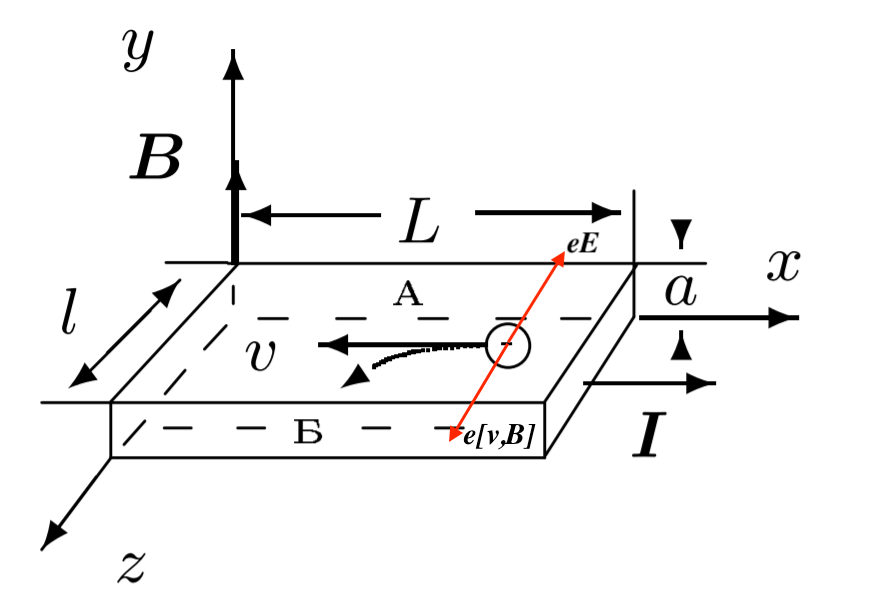
\includegraphics[width = 150pt]{image/Holl1.png}
    \caption{Образец с током в магнитном поле}
\end{figure}

	
	Если эту пластину поместить в магнитное поле, направленное по оси y, то между гранями А и Б появляется разность потенциалов. \medskip
	
	В самом деле, на электрон (для простоты рассматриваем один тип носителей), движущийся со средней скоростью $\langle \vec{v} \rangle$ в электромагнитном поле, действует сила Лоренца:
	
	$$\vec{F}_{\text{л}} = -e\vec{E}-e \langle \vec{v} \rangle \times \vec{B},$$
	
	где $e$ --- абсолютный заряд электрона, $\vec{E}$ --- напряженность электрического поля, $\vec{B}$~--- индукция магнитного поля. \medskip
	
	В проекции на ось $z$ получаем
	
	$$ F_{B}=e | \langle {v_{x}} \rangle | B.$$
	
	Под действием этой силы электроны отклоняются к грани Б, заряжая ее отрицательно. На грани А накапливаются нескомпенсированные положительные заряды. Это приводит к возникновению электрического поля $E_{z}$, направленного от А к Б, которое действует на электроны с силой $F_{E}=eE_{z}$. В установившемся режиме $F_{E}=F_{B}$, поэтому накопление электрических зарядов на боковых гранях пластины прекращается. Отсюда
	
	$$ E_{z}=| \langle {v_{x}} \rangle | B.$$
	
	С этим полем связана разность потенциалов $$U_{\text{AБ}}=E_{z}l=| \langle {v_{x}} \rangle | Bl.$$
	
	В этом и состоит эффект Холла. \medskip
	
	\noindent Замечая, что сила тока равна
	
	$$ I=ne| \langle {v_{x}} \rangle |la,$$
	
	найдем ЭДС Холла:
	
\begin{equation*}\label{Rx}
	\mathscr{E}_{X}=U_{\text{AБ}}=\dfrac{IB}{nea}=R_{X}\dfrac{IB}{a}.
\end{equation*}
	
	Константа $R_{X}=\dfrac{1}{ne}$ называется постоянной Холла. \medskip
	
	В полупроводниках, когда вклад в проводимость обусловлен и электронами и дырками, выражение для постоянной Холла имеет более сложный вид:
	
	$$R_{X}=\dfrac{nb^{2}_{e}-pb^{2}_{p}}{e(nb_{e}+pb_{p})^{2}},$$
	
	где $n$ и $p$ --- концентрации электронов и дырок, $b_{e}$ $b_{p}$ --- их подвижности.
	
	\subsection{Экспериментальная установка.}
	Схема экспериментальной установки показана на рис. 2.
	
	\begin{figure}[h!]
		\centering
		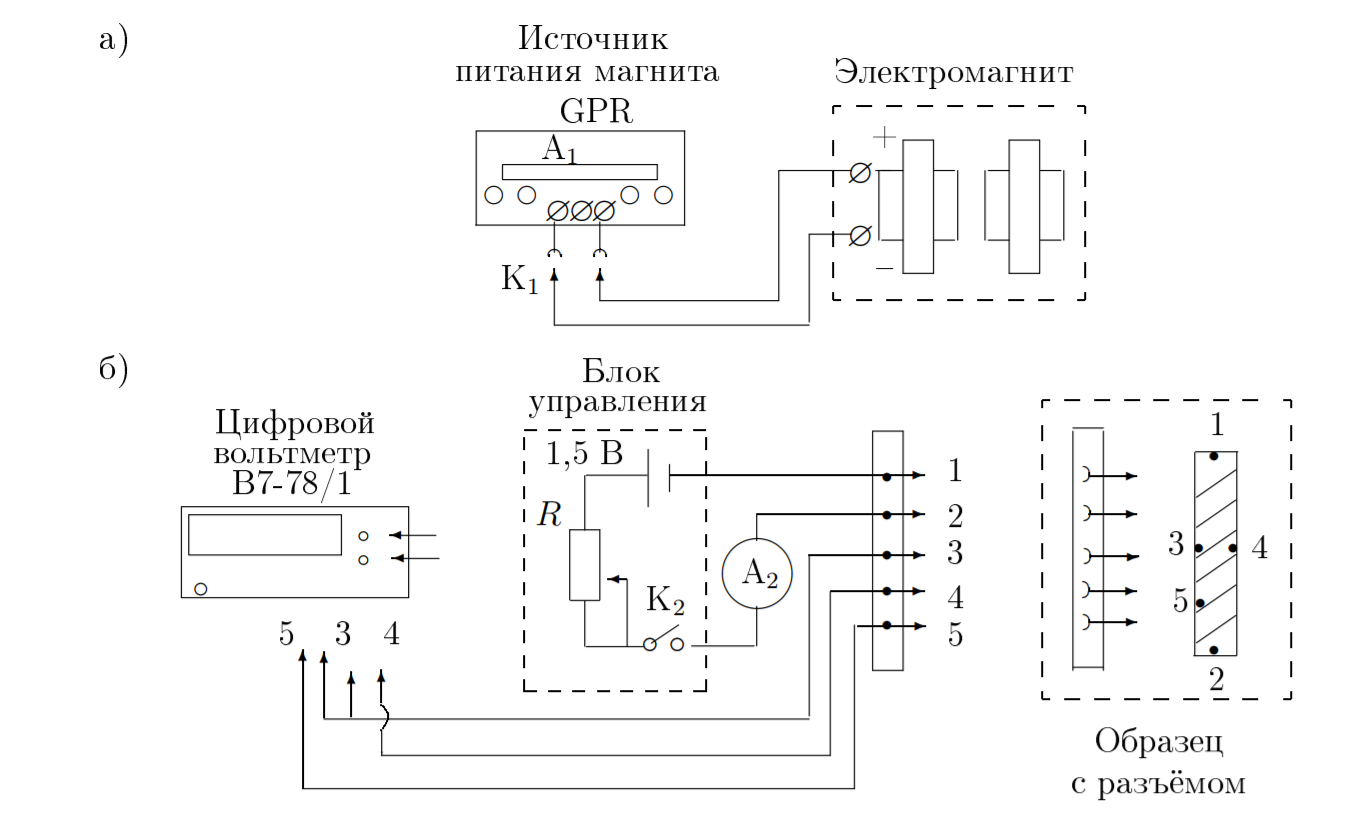
\includegraphics[width=\linewidth]{image/Holl2}
		\caption{Схема установки для исследования эффекта Холла в полупроводниках}
		\label{fig:Holl2}
	\end{figure}
  
  	В зазоре электромагнита (рис. 1а) создаётся постоянное магнитное поле, величину которого можно менять с помощью регуляторов источника питания. Ток измеряется амперметром источника питания $A_{1}$. Разъем $K_{1}$ позволяет менять направление тока в обмотках электромагнита. \medskip
  
  	Образец из легированного германия, смонтированный в специальном держателе (рис. 1б), подключается к батарее. При замыкании ключа $K_{2}$ вдоль длинной стороны образца течет ток, величина которого регулируется реостатом $R$ и измеряется миллиамперметром $A_{2}$. \medskip
  	
  	В образце с током, помещённом в зазор электромагнита, между контактами 3 и 4 возникает разность потенциалов $U_{34}$, которая измеряется с помощью цифрового вольтметра. \medskip
  	
  	Контакты 3 и 4 вследствие неточности подпайки не всегда лежат на одной
  	эквипотенциали, и тогда напряжение между ними связано не только с эффектом
  	Холла, но и с омическим падением напряжения, вызванным протеканием основного тока через образец. \medskip
  	
  	Измеряемая разность потенциалов при одном направлении
  	магнитного поля равна сумме ЭДС Холла и омического падения напряжения, а
  	при другом  их разности. В этом случае ЭДС Холла $\mathscr{E}_{X}$ может быть определена как половина алгебраической разности показаний вольтметра, полученных для
  	двух противоположных направлений магнитного поля в зазоре. \medskip
  	
  	Можно исключить влияние омического падения напряжения иначе, если при каждом токе через образец измерять напряжение между точками 3 и 4 в отсутствие магнитного поля. При фиксированном токе через образец это дополнительное к ЭДС Холла напряжение $U_{0}$ остается неизменным. От него следует (с учетом
  	знака) отсчитывать величину ЭДС Холла: 
  	
  	$$\mathscr{E}_{X} = U_{34} \pm U_{0}.$$
  	
  	При таком способе измерения нет необходимости проводить повторные измерения с противоположным направлением магнитного поля.
  	
  	
  	По знаку $\mathscr{E}_{X}$ можно определить характер проводимости - электронный или дырочный. Для этого необходимо знать направление тока в образце и направление
  	магнитного поля. \medskip
  	
  	Измерив ток $I$ в образце и напряжение $U_{35}$ между контактами 3 и 5 в отсутствие магнитного поля, можно, зная параметры образца, рассчитать проводимость материала образца по формуле:
  	
  \begin{equation*}
  	\sigma=\dfrac{IL_{35}}{U_{35}al}
  \end{equation*}
  	
  	где $L_{35}$ --- расстояние между контактами 3 и 5, $a$ - толщина образца, $l$ - его ширина.

\subsection{Формулы для расчёта}

\begin{itemize}
    \item
        ЭДС Холла:
        \begin{equation}
            \mathscr{E_\text{х}} = U_{34} - U_0;
        \end{equation}
    \item
        Постоянная Холла:
        \begin{equation}
            R_\text{х} = -\frac{\mathscr{E_\text{х}}}{B} \cdot \frac{a}{I};
        \end{equation}
    \item
        Концентрация носителей тока в образце:
        \begin{equation}
            n = \frac{1}{R_\text{х} e}
        \end{equation}
    \item
        Удельная проводимость материала образца:
        \begin{equation}
            \sigma = \frac{I L_{35}}{U_{35}al}
        \end{equation}
    \item
        Подвижность носителей тока:
        \begin{equation}
            b = \frac{\sigma}{en}
        \end{equation}
    
\end{itemize}

\section{Ход работы}

\begin{enumerate}
    \item Построим калибровочный график зависимости $B(I_M)$.
    \item Рассчитаем ЭДС Холла и построим семейство характеристик $U_{\bot}(B)$ при разных значениях тока $I$ через образец. Убедимся в линейности зависимостей и определим угловые коэффициенты $k = dU_{\bot} / dB$ полученных прямых.
    \item Построим график $k(I)$. Рассчитаем угловой коэффициент прямой и определим величину постоянной Холла.
    \item Рассчитаем концентрацию $n$ носителей тока в образце и удельную проводимость $\sigma_0$ материала.
    \item Используя найденные значения концентрации и удельной проводимости, вычислим подвижность $b$ носителей тока.
\end{enumerate}

\section{Результаты измерений и обработка данных}

    Исследуем зависимость потока $\Phi$ магнитного поля в зазоре электромагнита от тока через обмотки магнита. Данные занесём в таблицу 1. \medskip

    По этим данным построим график зависимости $B = B(I_M)$.

    \begin{figure}[h!]
        \centering
        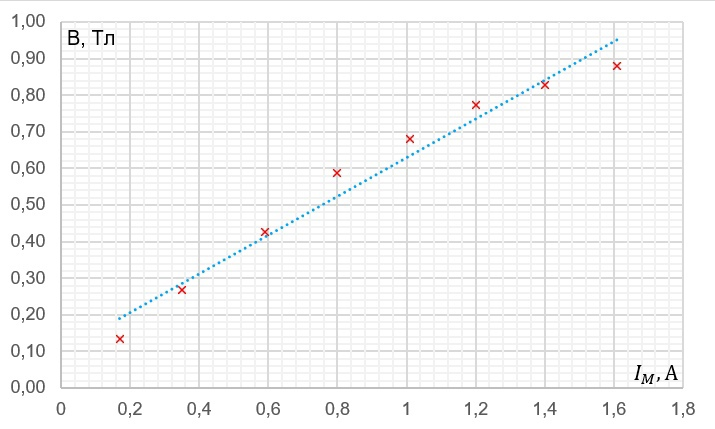
\includegraphics[width = 320pt]{image/graph1.jpg}
        \caption{График зависимости $B(I_M)$}
    \end{figure}

    \begin{table}[h!]
        \caption{}
        \centering
        \begin{tabular}{|c|c|c|}
        \hline
        \multicolumn{1}{|l|}{$I_M$, А} & \multicolumn{1}{l|}{$\Phi$, мВБ} & \multicolumn{1}{l|}{$B$, Т} \\ \hline
        0,17 & 1 & 0,13 \\ \hline
        0,35 & 2 & 0,27 \\ \hline
        0,59 & 3,2 & 0,43 \\ \hline
        0,80 & 4,4 & 0,59 \\ \hline
        1,01 & 5,1 & 0,68 \\ \hline
        1,20 & 5,8 & 0,77 \\ \hline
        1,40 & 6,2 & 0,83 \\ \hline
        1,61 & 6,6 & 0,88 \\ \hline
        \end{tabular}
        \end{table}

    Рассчитаем ЭДС Холла (таблица 3) и построим семейство характеристик $U(B)$ при разных значениях тока $I$ (рисунок 4).

    \begin{figure}[h!]
        \centering
        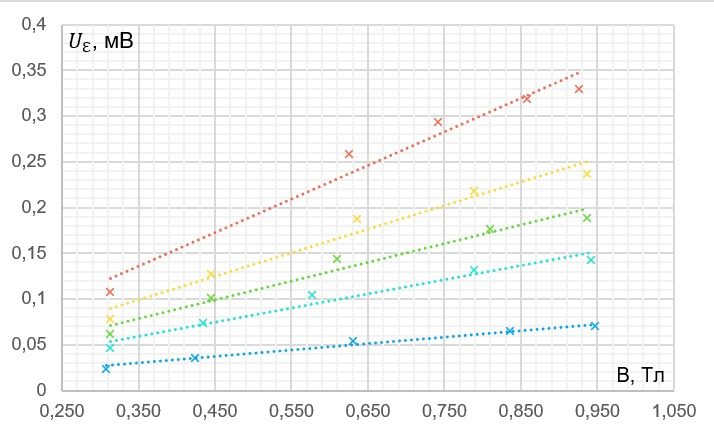
\includegraphics[width = 320pt]{image/graph2.jpg}
        \caption{График зависимости $U(B)$}
    \end{figure}

    Теперь по таблице 2 построим график зависимости $k(I)$.

    \begin{figure}[h!]
        \centering
        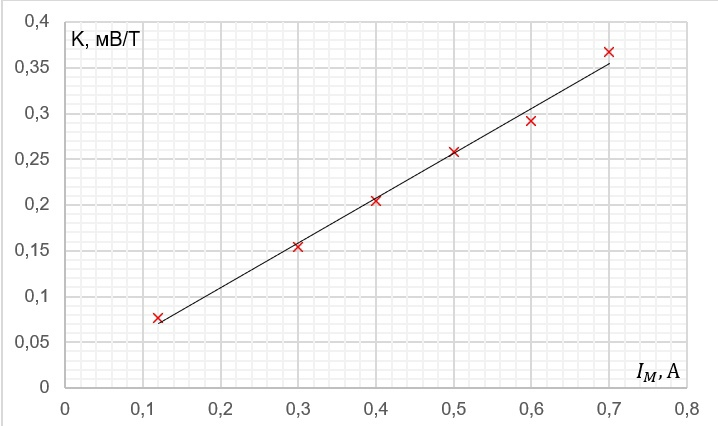
\includegraphics[width = 320pt]{image/graph3.jpg}
        \caption{График зависимости $U(B)$}
    \end{figure}

        \begin{table}[h!]
            \caption{}
            \centering
            \begin{tabular}{|c|c|}
            \hline
            \multicolumn{1}{|l|}{{$I_M$, мА}} & \multicolumn{1}{l|}{{$K$, мВ/Т}}\\ \hline
            0,12 & 0,0769 \\ \hline
            0,3 & 0,1542 \\ \hline
            0,4 & 0,2040 \\ \hline
            0,5 & 0,2574 \\ \hline
            0,6 & 0,2917 \\ \hline
            0,7 & 0,3676 \\ \hline
            -1,34 & -0,6548 \\ \hline
            \end{tabular}
            \end{table}

    Откуда можно найти постоянную Холла по формуле (2): $$R_{X} \approx (7,3 \pm 0,2)\cdot 10^{-4} \;\;\frac{\text{м}^3}{\text{Кл}}.$$

    Рассчитаем концентрацию $n$ носителей тока в образце и удельную проводимость $\sigma_0$ материала по формулам (3) и (4): $$n \approx (8,11 \pm 0,2) \cdot 10^{21} \;\;\frac{1}{\text{м}^3},$$ $$\sigma \approx 79, 8 \pm 0,6 \;\;(\text{Ом}\cdot\text{м})^{-1}.$$

    Теперь по формуле (5) рассчитаем подвижность носителей:

    $$b \approx 615 \pm 12 \;\;\frac{\text{см}^2}{\text{В}\cdot\text{с}}.$$

    \begin{figure}[h!]
        \caption*{Таблица 3}
        \centering
        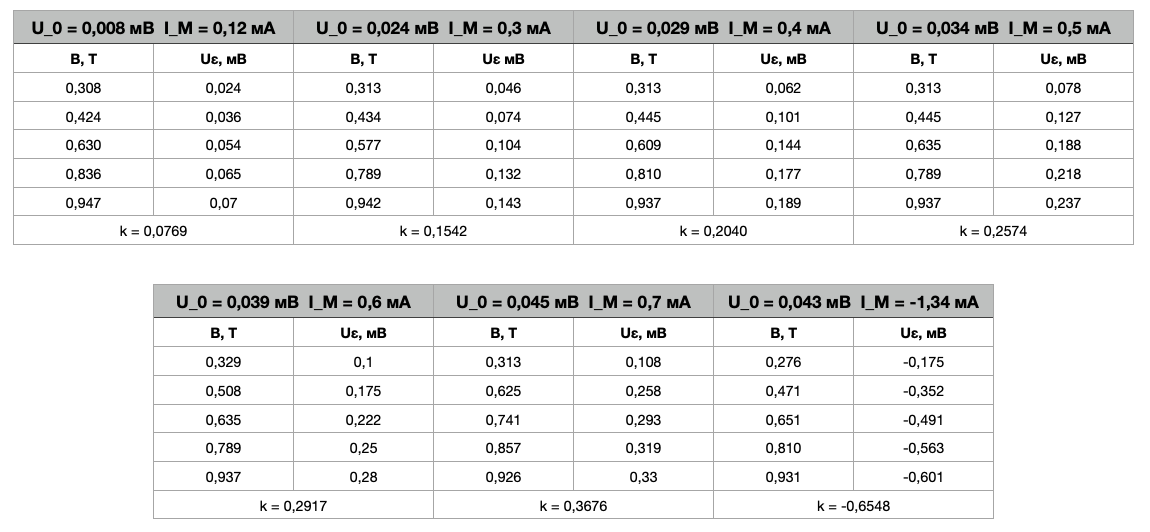
\includegraphics[width = 370pt]{image/table3.png}
    \end{figure}

    \section{Вывод}

    В ходе лабораторной работы был исследовали эффект Холла в полупроводнике --- германии. Удалось определить постоянную Холла, которая в данных диапазонах токов и значений магнитной индукции магнитного поля оказалась постоянной и равной $R_\text{х} = 730$ см$^3$/Кл. После чего была вычислена концентрация носителей тока в образце при предположении, что количество носителей одного типа намного больше другого: $n = 811\, \cdot \, 10^{19}\,\text{м}^{-3}$. \medskip
    
    Зная направление тока в проводнике, полярность вольтметра, направление тока в катушках, можно определить тип проводимости. В нашей работе тип проводимости в германии оказался дырочным. \medskip
	
	Более того, была вычислена подвижность дырок в исследуемом образце германия: $b = 615\, \frac{\text{см}^2}{\text{В}\cdot\text{с}}$. Полученный результат отличается от табличного для носителей в области собственной проводимости $b_0 = 1800\, \frac{\text{см}^2}{\text{В}\cdot\text{с}}$ (при температуре $T$ = 293 К), из чего можно сделать вывод, что образец содержит примеси. \medskip
    
    Дополнительная ошибка измерений может быть связана с сильной зависимостью концентрации основных носителей токов от температуры. Действительно, для отрыва электрона от атома полупроводника и превращения его в электрон проводимости необходимо сообщить ему некоторое колличество энергии. Естественно, что такая энергия поставляется тепловыми колебаниями атомов решетки. При выполнении работы температура образца была комнатной ($\approx 298$ К) и как могла повыситься вследствие протекающего через образец постоянного тока.
	

\end{document}
